\documentclass{article}

% if you need to pass options to natbib, use, e.g.:
%     \PassOptionsToPackage{numbers, compress}{natbib}
% before loading neurips_2020

% ready for submission
% \usepackage{neurips_2020}

% to compile a preprint version, e.g., for submission to arXiv, add add the
% [preprint] option:
\usepackage[preprint]{neurips_2020}

% to compile a camera-ready version, add the [final] option, e.g.:
%     \usepackage[final]{neurips_2020}

% to avoid loading the natbib package, add option nonatbib:
%     \usepackage[nonatbib]{neurips_2020}

\usepackage[utf8]{inputenc} % allow utf-8 input
\usepackage[T1]{fontenc}    % use 8-bit T1 fonts
\usepackage{hyperref}       % hyperlinks
\usepackage{url}            % simple URL typesetting
\usepackage{booktabs}       % professional-quality tables
\usepackage{amsfonts}       % blackboard math symbols
\usepackage{nicefrac}       % compact symbols for 1/2, etc.
\usepackage{microtype}      % microtypography
\usepackage{graphicx}

\title{Generation of Stereo Audio from a Mono Source Using
a Nearest-Neighbor Algorithm}

% The \author macro works with any number of authors. There are two commands
% used to separate the names and addresses of multiple authors: \And and \AND.
%
% Using \And between authors leaves it to LaTeX to determine where to break the
% lines. Using \AND forces a line break at that point. So, if LaTeX puts 3 of 4
% authors names on the first line, and the last on the second line, try using
% \AND instead of \And before the third author name.

\author{%
  Ethan James \\
  Virginia Tech\\
  \texttt{ethanjamesauto@vt.edu} \\
  % examples of more authors
  % \And
  % Coauthor \\
  % Affiliation \\
  % Address \\
  % \texttt{email} \\
  % \AND
  % Coauthor \\
  % Affiliation \\
  % Address \\
  % \texttt{email} \\
  % \And
  % Coauthor \\
  % Affiliation \\
  % Address \\
  % \texttt{email} \\
  % \And
  % Coauthor \\
  % Affiliation \\
  % Address \\
  % \texttt{email} \\
}

\begin{document}

\maketitle

\begin{abstract}
  This project presents a method of transforming mono audio tracks into stereo audio tracks using a K-Nearest Neighbor model in conjunction with a parametric stereo encoder/decoder used to decrease the problem's complexity. The implementations were created by implementing the model described in [1]. The model was trained on a dataset of 4000 30-second stereo audio tracks. The resulting model showed some signs of ability to generate stereo audio and results obtained are similar to [1]. All implementation source code is available at \url{https://github.com/ethanjamesauto/mono-to-stereo}.
\end{abstract}

\section{Problem Statement}
This project aims to create a trained model that transforms a mono (single-channel) audio track into a stereo (two-channel, left/right) audio track. This is accomplished by implemententing the model architecture described in [1]. This model implements the KNN (K-Nearest Neighbor) algorithm and uses an encoding/decoding scheme to convert a stereo audio track into data that may be more easily learned by a model.


\subsection{Parametric Stereo Encoder/Decoder}

The model's objective is to take a mono audio track $s[n]$ - a time series of digital audio samples at a sample rate $F_s=44100$ Hz - and generate two audio tracks $l[n]$ and $r[n]$, which also contain digital audio samples at the same sample rate. The model is trained on a dataset of stereo audio tracks, where the features are mono audio tracks created from those stereo audio tracks using the following transformation:
$$s = \frac{l+r}{2}$$
and the labels are the stereo tracks themselves. This makes finding a dataset simple - find a database of stereo audio tracks, convert them to mono, and train the model on the mono and stereo tracks.

Training a model to directly accomplish this task would be extremely difficult - the model would have to learn to generate two audio tracks from one. Instead, the stereo audio tracks are converted into a \textbf{parametric representation}, where a stereo track is represented as a mono track and additional data that encodes the stereo information. This way, the model's features are mono audio tracks and the model's label is the parametric stereo information. The stereo information along with the original mono source are then decoded into a stereo audio track. This stereo information is in the form of a spectrogram - a 2D array containing frequency information over time, generated using many short FFTs (Fast Fourier Transforms) over the audio track. This stereo information takes up only about 5\% of the space of the original stereo audio track and separates the information into discrete frequency bands, making it easier for the model to learn.

I implemented this encoder/decoder in Python using NumPy and some SciPy (for Short-Time FFT, filtering, etc). The encoder is implemented in an identical fashion to [1], and the decoder is implemented using [2]. This was done because [1] describes a KNN that uses the decoder described in [2], but [1] only describes the encoder and references [2] for the decoder. The encoder outputs parametric stereo parameters for a stereo track, which is used during training time to generate the labels for the model. The decoder is used at all times to convert the parametric stereo information (along with the mono source) into a stereo audio track.

The encoder and decoder are implemented using vectorized functions and are robust and quite fast as a result. They are implemented as two Python functions:

\begin{verbatim}
[l, r] = decode(s, P_IID, P_IC)
[P_IID, P_IC] = encode(l, r)
\end{verbatim}

where $l$ and $r$ are the left and right channels of the stereo audio track, and $P_{IID}$ and $P_{IC}$ are the parametric stereo parameters - $P_{IID}$ represents the difference in intensity between the left and right channels, and $P_{IC}$ represents the difference in phase.

\subsection{K-Nearest Neighbor Algorithm}
The KNN regressor outlined in [1] is a 1-nearest neighbor that takes in some frames of the \textbf{spectrogram} of the mono audio source and outputs the estimated corresponding pa rametric stereo data for the last frame. Note that the spectrogram is generated with window size $N=4096$, overlapping windows with 75\% overlap, and a Hann window applied to each frame. I implemented this KNN using scikit-learn's KNeighborsRegressor, and trained the model on a small dataset of stereo audio tracks from the FMA dataset [3].

The model architecture is shown below for both training and prediction:
\begin{center}
  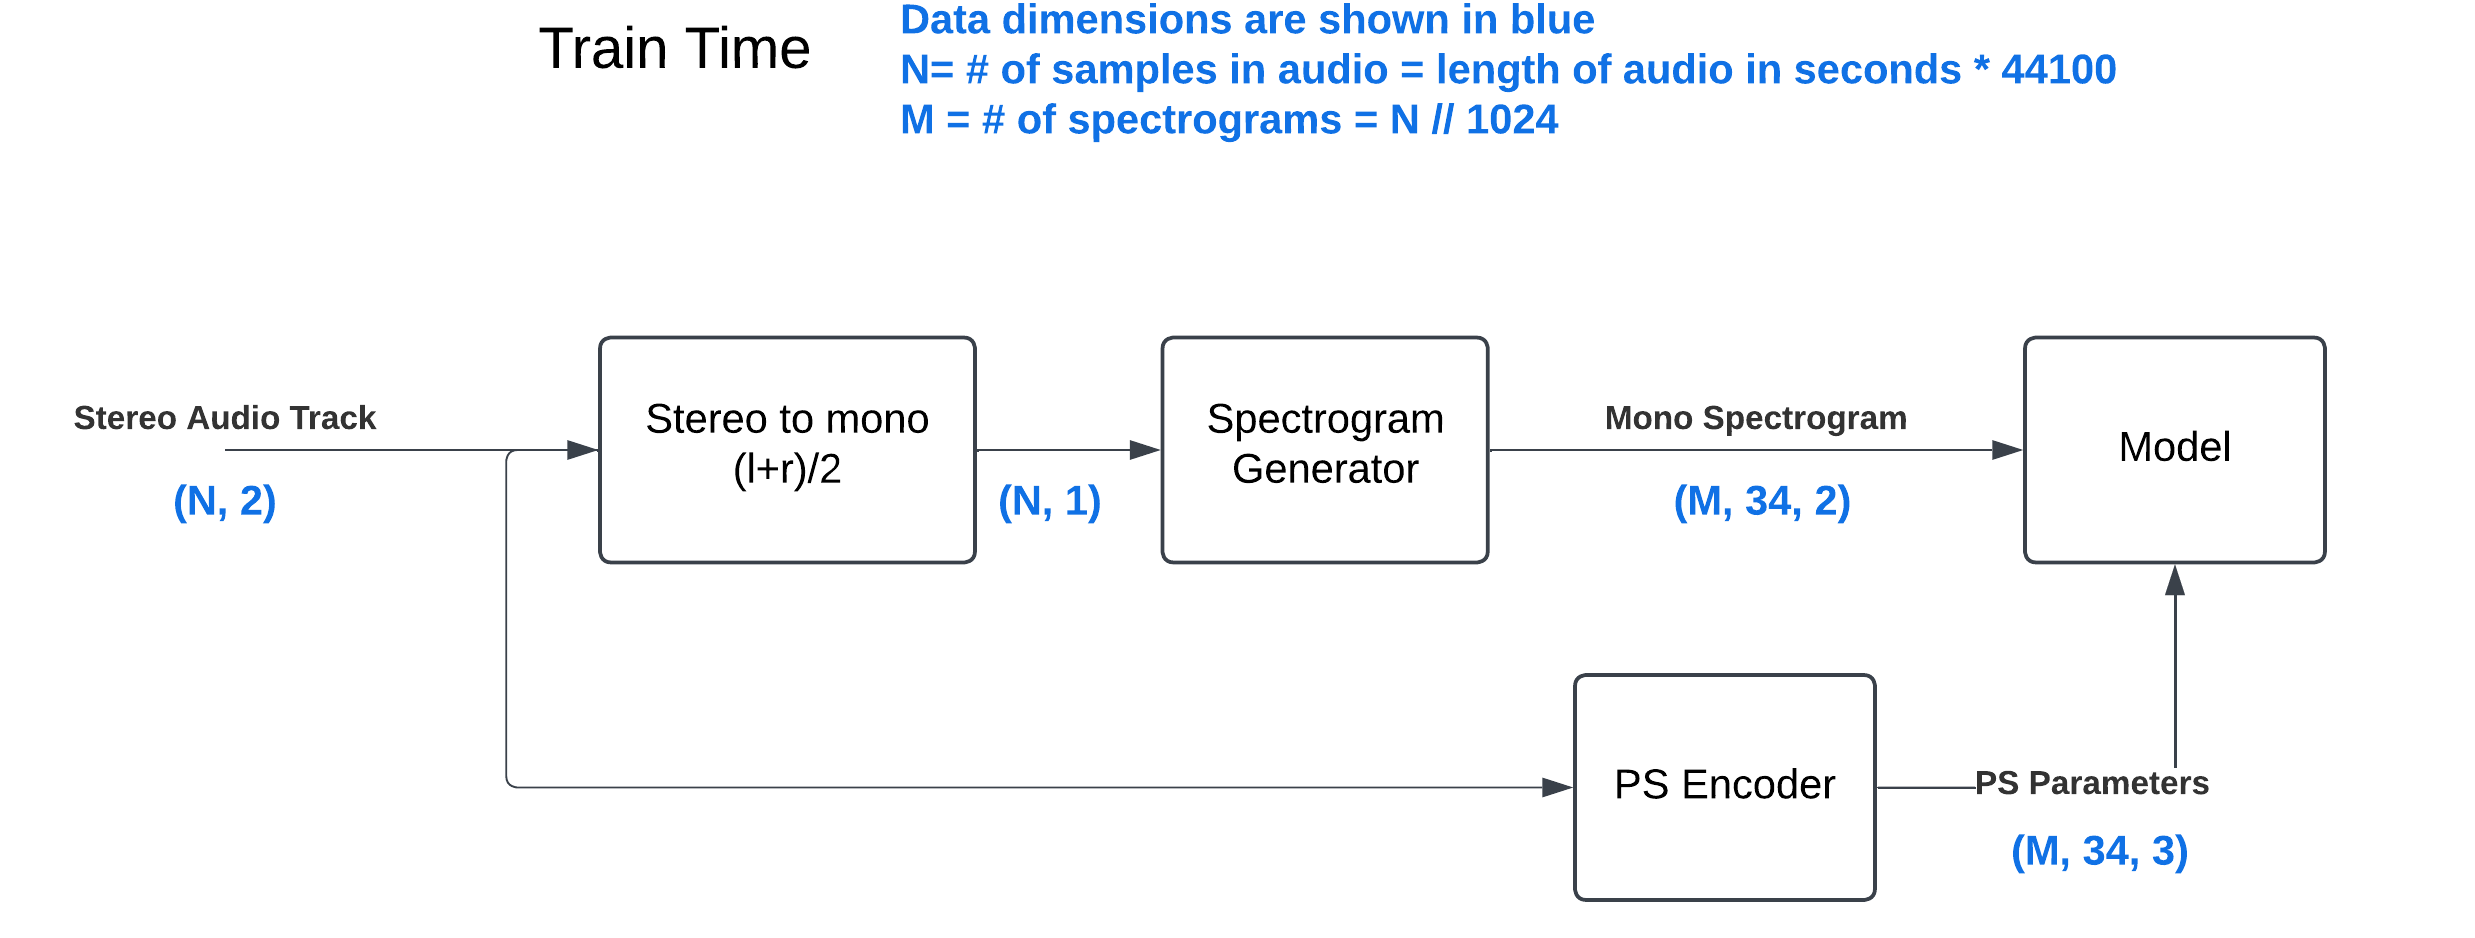
\includegraphics[width=1.0\textwidth]{train.png}
\end{center}

\begin{center}
  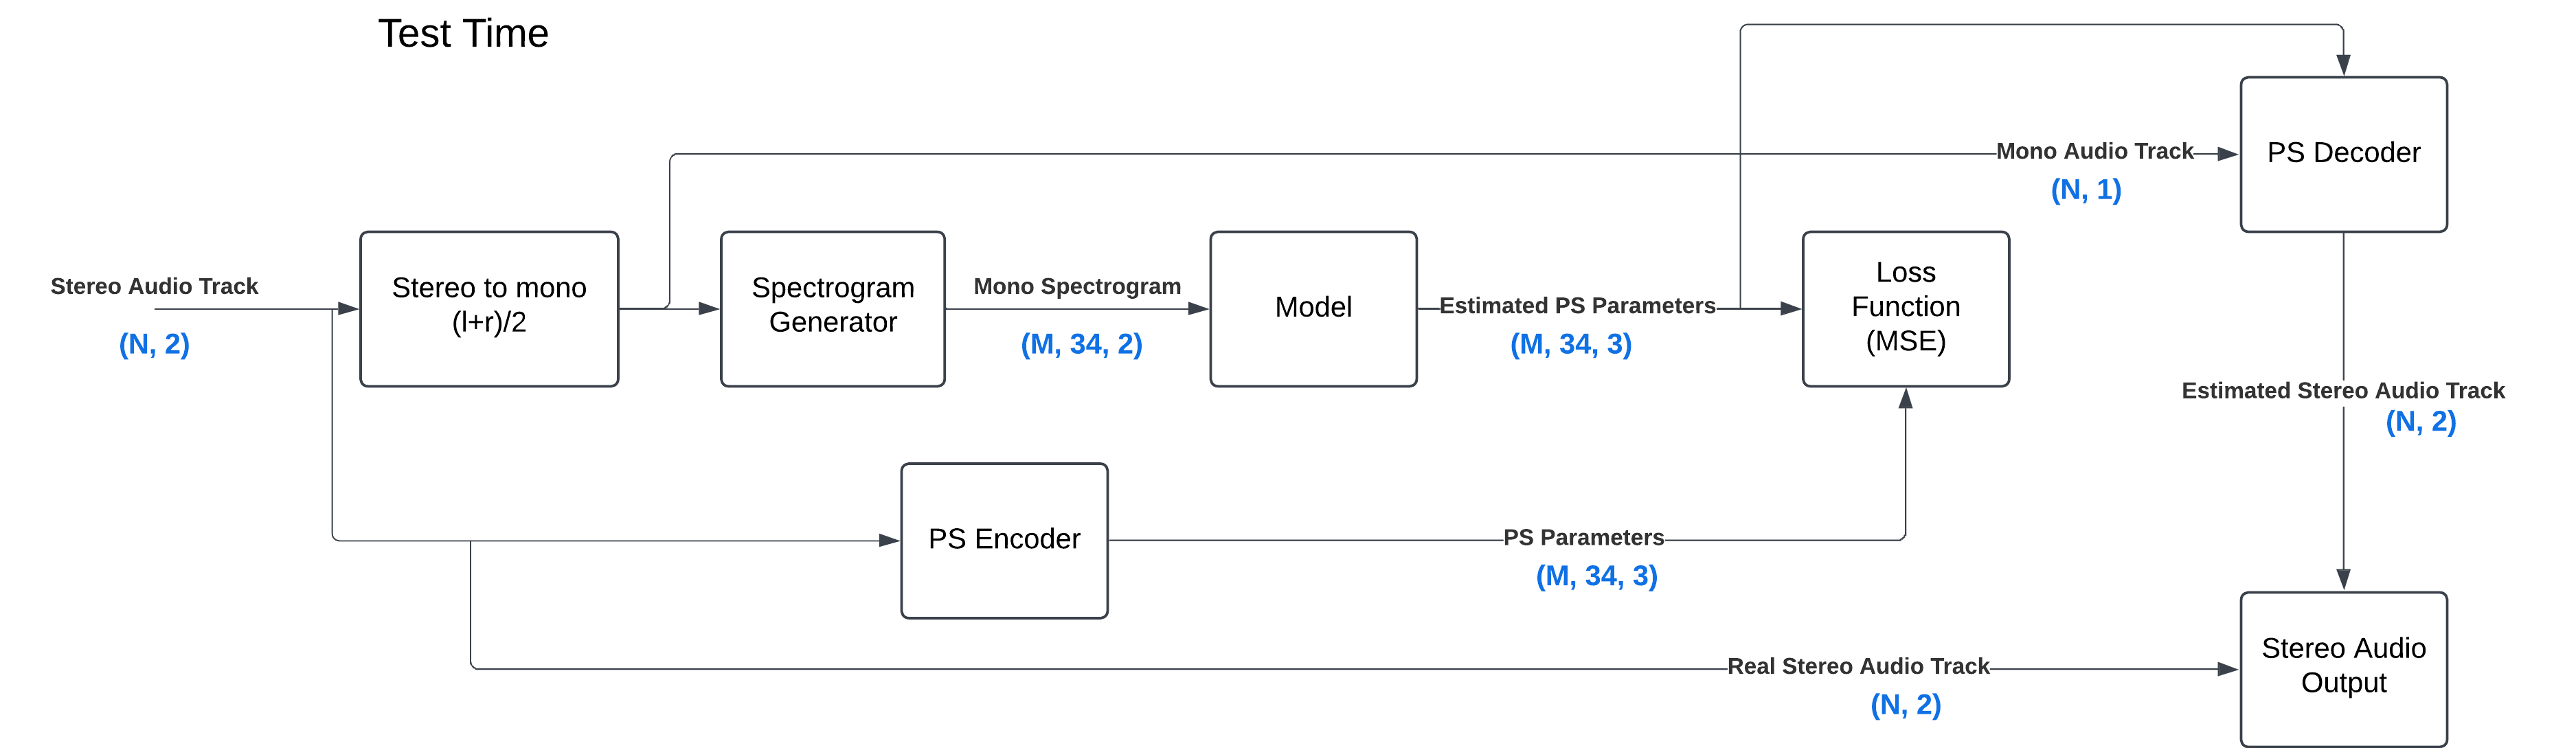
\includegraphics[width=1.0\textwidth]{test.png}
\end{center}

\subsubsection{Training}
The model is trained by repeating the following procedure:
\begin{enumerate}
  \item Randomly select a stereo audio track from the dataset
  \item Pick a random $N=20$ consecutive frames from the spectrogram of the audio track downmixed to mono
  \item Place the frames in the KNN structure as a feature, and place the parametric stereo data from the last frame as the label
\end{enumerate}

This process is used to allow the KNN to predict a time series - the input is contains the frames from about a second of audio, and the output is the parametric stereo data for the final frame.

Similar to the procedure described in [1], I repeated this process half a million times. The original paper notes this number of iterations, but it did not state the amount of audio tracks used in training. I trained the model on approximately 4000 30-second stereo audio tracks from the FMA dataset [3], using an 80/20 train/test split.

\subsubsection{Prediction}
The model is used to convert a mono track to stereo by first taking the spectrogram of the mono track with the aforementioned parameters ($N=4096$, etc). For every frame in the spectrogram, 20 frames are taken and inputted into the KNN. The output of the KNN is the parametric stereo data for the last frame. This data is then decoded into a coherent stereo track.

\section{Results}

As previously mentioned, the model was trained on a dataset of stereo audio tracks with an 80/20 testing split. Below is a table containing the mean-squared error of the model on the test and training sets, in addition to the baseline error - that is, the error of the mono audio track before attempting to convert it to stereo.

\begin{center}
  \begin{tabular}{ |c|c|c|c| } 
   \hline
   & Baseline Error & KNN Output Error \\ 
   \hline
   Training & 18.26 & 36.35 \\ 
   \hline
   Testing & 17.28 & 40.12 \\ 
   \hline
  \end{tabular}
\end{center}

As shown above, the model actually increases the error of the audio track, which indicates that the model does not converge to a useable solution. To investigate this further, I have included two spectrogram plots, where the top plot is the real parametric stereo data, and the bottom plot is the output of the KNN. The plots are from the same audio track, and the KNN output is from the test set:

\begin{center}
  \includegraphics[width=1.0\textwidth]{data.PNG}
\end{center}

It appears that while the KNN seems to have some idea of the stereo information, it will occasionally output stereo information that is not coherent with the previous frames. When the audio tracks are listened to, this phenomenon is very apparent - the audio rapidly oscillates between the left and right channels.


\section{Interpretation of Results}
The data presented in the previous section strongly indicates that the KNN Regressor does not converge to a useable solution. However, it appears that the authors of the original paper came to a similar conclusion - they noted that filtering was needed to stop the model from outputting audio that rapidly oscillated between the left and right channels, which is a sign of model confusion. Additionally, they did not use the mean-squared error metric to compute error - instead, they reported the 
\textbf{minimum error across all frames of the audio track} - the error of the best-case result out of each audio track's ~1300 total frames. While I will not directly challenge the results of the original paper (I'm scared of the implications), I will note that this error metric is not standard and provides almost no insight into the model's performance.

While I cannot provide a useable model that converts mono audio to stereo audio, I can provide insight into why the model failed to converge, and what steps can be taken to create a working model. Firstly - there are most certainly better models to use than a KNN - namely models that work well with time series data. Because the KNN can only output a single frame of audio at one time, it's likely that the following audio frame will not be coherent with the previous frame. This is likely the cause of the rapid oscillation between left and right channels. A model that can output multiple frames at once, such as an RNN or a CNN, would likely perform better.

Additionally, it might be the case that this task is more suited to a generative model. This is because the correlation between the mono and stereo audio tracks is quite low, as there many stereo representations for each mono track. A generative model could create one of these stereo representations, and a sufficiently trained model could create a very convincing stereo audio track. 

\section*{References}

\small

[1] MONO-TO-STEREO THROUGH PARAMETRIC STEREO GENERATION

\url{https://arxiv.org/pdf/2306.14647}


[2] Parametric Coding of Stereo Audio

\url{https://asp-eurasipjournals.springeropen.com/articles/10.1155/ASP.2005.1305}

[3] FMA: A Dataset For Music Analysis

\url{https://github.com/mdeff/fma}

\end{document}
